\documentclass[../main.tex]{subfiles}
\graphicspath{{\subfix{images/}}}

\begin{document}

\section{Results}

\subsection{The recommended content}

\subsection{Leaving the filter bubble}

\subsection{Machine learning}

\begin{figure}[t!]
  \textbf{Classifier performance}\par\medskip
  \centering
  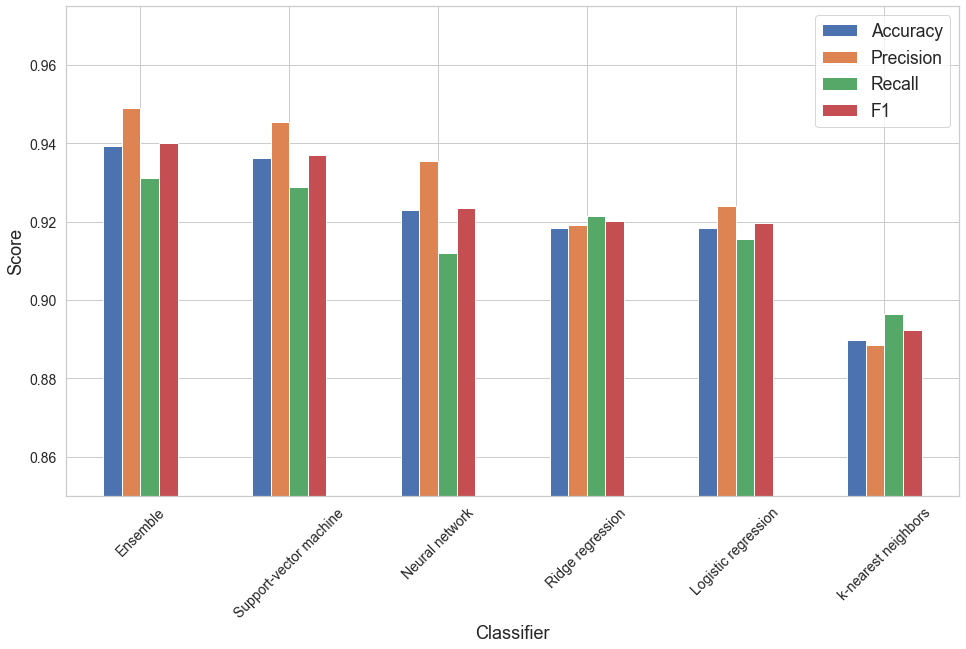
\includegraphics[keepaspectratio, width=\textwidth]{images/classifier_results.png}
  \caption{Metrics for each classifier with optimized hyperparameters}
  \label{fig:ML_scores}
\end{figure}

The hyperparameter tuning lead to impressive scores for all classifiers. The best-performing classifier is the support-vector machine making use of the Radial Basis Function (RBF) kernel and a penalty parameter (C-value) of 10. The SVM is closely followed by the neural network using the identity activation function, with 10 hidden layers of 10 neurons. In third place, there is a two-way tie for accuracy between ridge regression with a sparse-cg solver and penalty (alpha) value of 0.1, and logistic regression with an L2 penalty, a penalty (C) value of 20 and a newton-cg solver. However, ridge regression has a slightly better F1-score, though this difference is neglectable (0.9202 as opposed to 0.9197). The worst-performing classifier is also the simplest of the bunch: the k-nearest neighbors classifier (K=1). Although its performance is still formidable, it does substantially worse than the others. An overview of all metrics for each classifier can be seen in figure \ref{fig:ML_scores}. The ten best-performing configurations for each classifier can be found in section \ref{Appendix 1}.

Noteworthy is the fact that the optimal ensemble actually outperforms the support-vector machine by a slight margin. This ensemble, consisting of the SVM, the neural network, and surprisingly, the k-nearest neighbor classifiers, gets slightly higher scores than the runner-up across the board. The ensemble had a 16-way tie for best-performing parameters, all of which contained at least the SVM, neural network, and k-NN classifiers. 

Though the ensemble outperforms the other classifiers, it has a significant drawback: its training time is significantly larger than that of the individual classifiers. Support-vector machines are infamous for their slowness when there is a lot of training data, and neural networks can require a lot of training time whenever the number of neurons gets large \citep{burges1997improving, kamarthi1999accelerating}. Requiring both algorithms to run will therefore require a lot of additional training time. Considering the marginal performance increase, the cost outweighs the benefit. As a result, when taking everything into account, the support-vector machine is the best classifier for labeling conspiracy videos on YouTube.  

\end{document}